\documentclass[]{report}
\usepackage[utf8]{inputenc}
\usepackage{geometry}
\geometry{a4paper,left=2cm,right=3cm, top=2cm, bottom=2cm} 


\usepackage{amsmath}
\usepackage{siunitx}
\usepackage{graphicx}
\usepackage{caption}
\usepackage{subcaption}

\usepackage{pgfplots}
% and optionally (as of Pgfplots 1.3):
\pgfplotsset{compat=newest}
\pgfplotsset{plot coordinates/math parser=false}
\newlength\figureheight
\newlength\figurewidth 
\setlength\figureheight{5cm}
\setlength\figurewidth{\textwidth}


\renewcommand\floatpagefraction{.99}


% Title Page
\title{Gruppennummer 16}
\author{Andreas Cremer (0926918)\\Hanna Huber (0925230) \\Lena Trautmann (1526567)}



\begin{document}
	\maketitle
	
	%\begin{abstract}
	%\end{abstract}
	
	\begin{enumerate}
		\item Shape-Modell \\\\
			Abbildung~\ref{fig:trafo} zeigt von generateShape.m generierte Shapes und vergleicht die Original-Shape mit verschiedenen Transformationen.
			\setlength\figureheight{3.5cm}
			\setlength\figurewidth{.4\textwidth}
			\begin{figure}
				\begin{subfigure}{0.45\textwidth}
					\centering
					% This file was created by matlab2tikz.
% Minimal pgfplots version: 1.3
%
%The latest updates can be retrieved from
%  http://www.mathworks.com/matlabcentral/fileexchange/22022-matlab2tikz
%where you can also make suggestions and rate matlab2tikz.
%
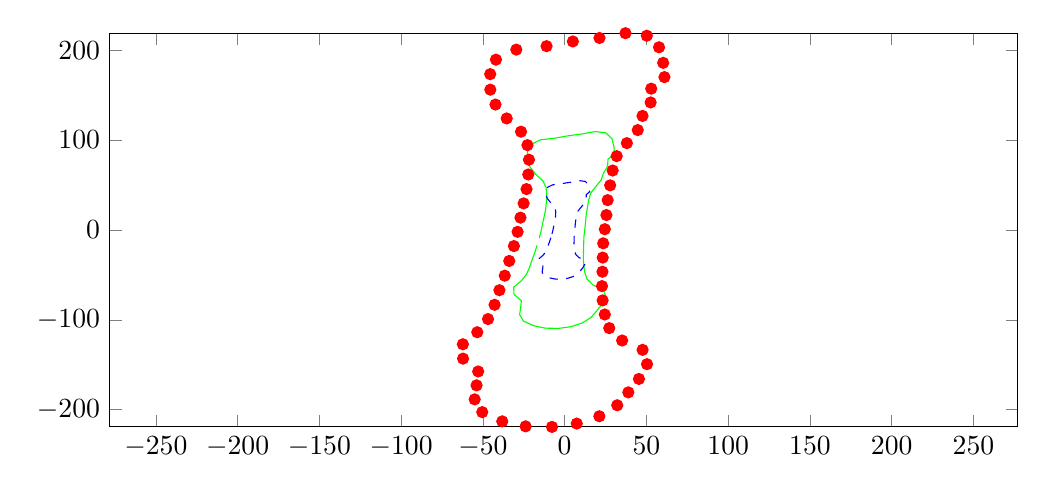
\begin{tikzpicture}

\begin{axis}[%
width=0.95092\figurewidth,
height=\figureheight,
at={(0\figurewidth,0\figureheight)},
scale only axis,
separate axis lines,
every outer x axis line/.append style={black},
every x tick label/.append style={font=\color{black}},
xmin=-278.198169217876,
xmax=276.965569773693,
every outer y axis line/.append style={black},
every y tick label/.append style={font=\color{black}},
ymin=-219.078104033269,
ymax=218.784909461694
]
\addplot [color=green,solid,forget plot]
  table[row sep=crcr]{%
-16.9383008024585	-17.2540700419669\\
-18.3191546519567	-25.4359033790996\\
-19.9491020291355	-33.5312106952851\\
-21.4291189738092	-41.6332714839577\\
-23.4325934348993	-49.5825754086476\\
-26.7176285471632	-56.8943991598107\\
-31.1267949632225	-63.5860197531732\\
-31.0704497227118	-71.5674748745803\\
-26.4379811698871	-78.7151426511731\\
-26.9284073326641	-86.4232733437989\\
-27.5110893006216	-94.2182867904342\\
-25.1979225333846	-101.328977289501\\
-19.0786164239692	-106.458107909618\\
-11.9329700175712	-109.235419234112\\
-3.87185321948764	-109.539052016635\\
3.69595476934701	-107.694550034826\\
10.6040509809237	-103.610505689942\\
16.0738264182722	-97.5033072431341\\
19.4667298360072	-90.3323944289307\\
22.7118143384688	-82.8716003330266\\
25.1758355250203	-74.6529650067753\\
23.8318526210809	-66.6897319700684\\
17.5728140268441	-61.4916681638731\\
13.6357941739749	-54.6124247953319\\
12.2743466048961	-47.0227345980446\\
11.6053154311707	-39.1855081988353\\
11.4141254579142	-31.2468930073932\\
11.5508054391741	-23.2526358624026\\
11.6382748738122	-15.3810106226617\\
11.7862124201461	-7.44925402870258\\
12.2836207078492	0.408014023438319\\
12.764595432433	8.27040489118245\\
13.1459674974322	16.5683453024354\\
13.914944379972	24.7830543694155\\
14.6768488234752	33.0339986121794\\
15.9132711362889	41.0247575333806\\
19.0171378907613	48.2554620111854\\
22.3522725115161	55.5234846116251\\
23.8081395520568	63.3970336029318\\
26.2875145747278	70.892388597312\\
26.4645056213721	78.5519041188589\\
30.5104952411306	84.9694154986342\\
30.1178420665977	92.9115504342284\\
28.8517396683747	101.570102952583\\
25.1130491911448	107.995981860857\\
18.5884874875498	109.392454730847\\
10.6498659785291	106.739128233057\\
2.50383074847667	104.799129433769\\
-5.53504215733932	102.184734870287\\
-14.7813514194023	100.254498070884\\
-21.0049392171998	94.6760255214926\\
-22.7604403189108	86.62589780194\\
-22.7256966435158	77.9871674146514\\
-21.1470194611919	69.7081370790496\\
-17.7203358905016	62.0065646594886\\
-13.3397436214445	54.6264358822352\\
-11.3752111213659	47.1455296342044\\
-10.9180819392748	39.0335197567964\\
-11.1341721230248	30.8260313769864\\
-11.6566897428528	22.7037005494587\\
-12.5495998431267	14.7548011008601\\
-13.51112615278	6.82423225112747\\
-14.3842506054937	-1.06404766792365\\
-15.5164439615494	-8.98008173430333\\
};
\addplot [color=red,only marks,mark=*,mark options={solid},forget plot]
  table[row sep=crcr]{%
-33.8766016049169	-34.5081400839337\\
-36.6383093039134	-50.8718067581992\\
-39.8982040582711	-67.0624213905703\\
-42.8582379476183	-83.2665429679154\\
-46.8651868697986	-99.1651508172952\\
-53.4352570943264	-113.788798319621\\
-62.2535899264449	-127.172039506346\\
-62.1408994454236	-143.134949749161\\
-52.8759623397741	-157.430285302346\\
-53.8568146653282	-172.846546687598\\
-55.0221786012432	-188.436573580868\\
-50.3958450667692	-202.657954579001\\
-38.1572328479383	-212.916215819236\\
-23.8659400351424	-218.470838468224\\
-7.74370643897529	-219.078104033269\\
7.39190953869403	-215.389100069653\\
21.2081019618474	-207.221011379884\\
32.1476528365444	-195.006614486268\\
38.9334596720144	-180.664788857861\\
45.4236286769376	-165.743200666053\\
50.3516710500406	-149.305930013551\\
47.6637052421617	-133.379463940137\\
35.1456280536882	-122.983336327746\\
27.2715883479498	-109.224849590664\\
24.5486932097922	-94.0454691960893\\
23.2106308623415	-78.3710163976706\\
22.8282509158284	-62.4937860147865\\
23.1016108783483	-46.5052717248051\\
23.2765497476244	-30.7620212453234\\
23.5724248402923	-14.8985080574052\\
24.5672414156984	0.816028046876637\\
25.529190864866	16.5408097823649\\
26.2919349948644	33.1366906048709\\
27.8298887599441	49.566108738831\\
29.3536976469505	66.0679972243588\\
31.8265422725779	82.0495150667611\\
38.0342757815227	96.5109240223707\\
44.7045450230322	111.04696922325\\
47.6162791041137	126.794067205864\\
52.5750291494556	141.784777194624\\
52.9290112427442	157.103808237718\\
61.0209904822611	169.938830997268\\
60.2356841331954	185.823100868457\\
57.7034793367495	203.140205905166\\
50.2260983822897	215.991963721714\\
37.1769749750995	218.784909461694\\
21.2997319570582	213.478256466114\\
5.00766149695335	209.598258867538\\
-11.0700843146786	204.369469740574\\
-29.5627028388045	200.508996141768\\
-42.0098784343997	189.352051042985\\
-45.5208806378216	173.25179560388\\
-45.4513932870316	155.974334829303\\
-42.2940389223839	139.416274158099\\
-35.4406717810032	124.013129318977\\
-26.6794872428889	109.25287176447\\
-22.7504222427319	94.2910592684089\\
-21.8361638785496	78.0670395135928\\
-22.2683442460496	61.6520627539729\\
-23.3133794857057	45.4074010989174\\
-25.0991996862533	29.5096022017202\\
-27.0222523055601	13.6484645022549\\
-28.7685012109875	-2.1280953358473\\
-31.0328879230989	-17.9601634686067\\
};
\addplot [color=blue,dashed,forget plot]
  table[row sep=crcr]{%
-8.46915040122923	-8.62703502098343\\
-9.15957732597836	-12.7179516895498\\
-9.97455101456777	-16.7656053476426\\
-10.7145594869046	-20.8166357419788\\
-11.7162967174496	-24.7912877043238\\
-13.3588142735816	-28.4471995799053\\
-15.5633974816112	-31.7930098765866\\
-15.5352248613559	-35.7837374372902\\
-13.2189905849435	-39.3575713255865\\
-13.464203666332	-43.2116366718994\\
-13.7555446503108	-47.1091433952171\\
-12.5989612666923	-50.6644886447503\\
-9.53930821198458	-53.2290539548089\\
-5.9664850087856	-54.6177096170559\\
-1.93592660974382	-54.7695260083173\\
1.84797738467351	-53.8472750174131\\
5.30202549046185	-51.805252844971\\
8.03691320913609	-48.751653621567\\
9.7333649180036	-45.1661972144653\\
11.3559071692344	-41.4358001665133\\
12.5879177625102	-37.3264825033877\\
11.9159263105404	-33.3448659850342\\
8.78640701342204	-30.7458340819366\\
6.81789708698744	-27.306212397666\\
6.13717330244804	-23.5113672990223\\
5.80265771558536	-19.5927540994176\\
5.7070627289571	-15.6234465036966\\
5.77540271958707	-11.6263179312013\\
5.8191374369061	-7.69050531133085\\
5.89310621007307	-3.72462701435129\\
6.14181035392461	0.204007011719159\\
6.38229771621651	4.13520244559123\\
6.5729837487161	8.28417265121771\\
6.95747218998602	12.3915271847078\\
7.33842441173762	16.5169993060897\\
7.95663556814447	20.5123787666903\\
9.50856894538067	24.1277310055927\\
11.1761362557581	27.7617423058126\\
11.9040697760284	31.6985168014659\\
13.1437572873639	35.446194298656\\
13.232252810686	39.2759520594294\\
15.2552476205653	42.4847077493171\\
15.0589210332988	46.4557752171142\\
14.4258698341874	50.7850514762915\\
12.5565245955724	53.9979909304286\\
9.29424374377488	54.6962273654236\\
5.32493298926456	53.3695641165286\\
1.25191537423834	52.3995647168845\\
-2.76752107866966	51.0923674351434\\
-7.39067570970113	50.1272490354421\\
-10.5024696085999	47.3380127607463\\
-11.3802201594554	43.31294890097\\
-11.3628483217579	38.9935837073257\\
-10.573509730596	34.8540685395248\\
-8.8601679452508	31.0032823297443\\
-6.66987181072223	27.3132179411176\\
-5.68760556068297	23.5727648171022\\
-5.45904096963741	19.5167598783982\\
-5.5670860615124	15.4130156884932\\
-5.82834487142642	11.3518502747293\\
-6.27479992156333	7.37740055043005\\
-6.75556307639002	3.41211612556374\\
-7.19212530274687	-0.532023833961825\\
-7.75822198077471	-4.49004086715166\\
};
\end{axis}
\end{tikzpicture}%
					\caption{$s=2$ (rot) und $s=0.5$ (blau)}
					\label{fig:s}
				\end{subfigure}
				\qquad
				\begin{subfigure}{0.45\textwidth}
					\centering
					% This file was created by matlab2tikz.
% Minimal pgfplots version: 1.3
%
%The latest updates can be retrieved from
%  http://www.mathworks.com/matlabcentral/fileexchange/22022-matlab2tikz
%where you can also make suggestions and rate matlab2tikz.
%
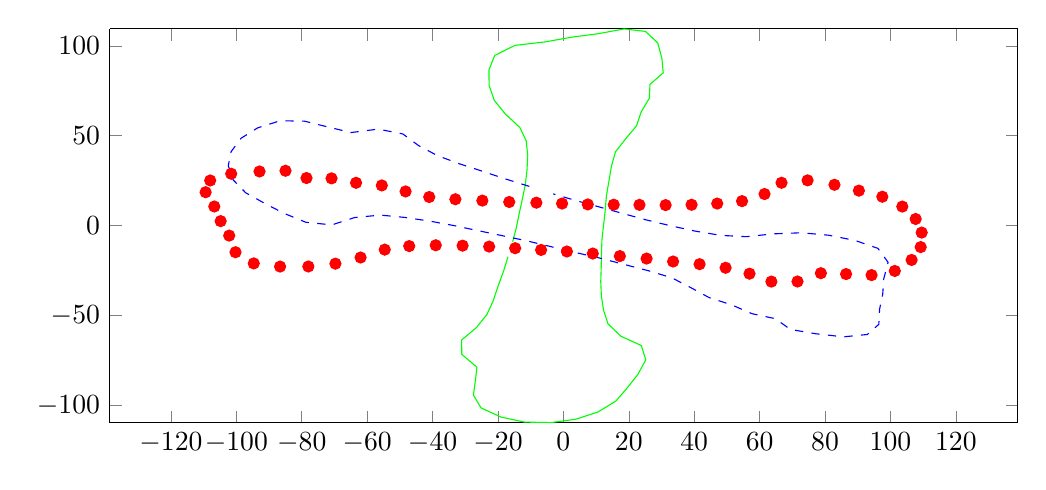
\begin{tikzpicture}

\begin{axis}[%
width=0.95092\figurewidth,
height=\figureheight,
at={(0\figurewidth,0\figureheight)},
scale only axis,
separate axis lines,
every outer x axis line/.append style={black},
every x tick label/.append style={font=\color{black}},
xmin=-138.717636104999,
xmax=138.864233390786,
every outer y axis line/.append style={black},
every y tick label/.append style={font=\color{black}},
ymin=-109.539052016634,
ymax=109.392454730847
]
\addplot [color=green,solid,forget plot]
  table[row sep=crcr]{%
-16.9383008024585	-17.2540700419669\\
-18.3191546519567	-25.4359033790996\\
-19.9491020291355	-33.5312106952851\\
-21.4291189738092	-41.6332714839577\\
-23.4325934348993	-49.5825754086476\\
-26.7176285471632	-56.8943991598107\\
-31.1267949632225	-63.5860197531732\\
-31.0704497227118	-71.5674748745803\\
-26.4379811698871	-78.7151426511731\\
-26.9284073326641	-86.4232733437989\\
-27.5110893006216	-94.2182867904342\\
-25.1979225333846	-101.328977289501\\
-19.0786164239692	-106.458107909618\\
-11.9329700175712	-109.235419234112\\
-3.87185321948764	-109.539052016635\\
3.69595476934701	-107.694550034826\\
10.6040509809237	-103.610505689942\\
16.0738264182722	-97.5033072431341\\
19.4667298360072	-90.3323944289307\\
22.7118143384688	-82.8716003330266\\
25.1758355250203	-74.6529650067753\\
23.8318526210809	-66.6897319700684\\
17.5728140268441	-61.4916681638731\\
13.6357941739749	-54.6124247953319\\
12.2743466048961	-47.0227345980446\\
11.6053154311707	-39.1855081988353\\
11.4141254579142	-31.2468930073932\\
11.5508054391741	-23.2526358624026\\
11.6382748738122	-15.3810106226617\\
11.7862124201461	-7.44925402870258\\
12.2836207078492	0.408014023438319\\
12.764595432433	8.27040489118245\\
13.1459674974322	16.5683453024354\\
13.914944379972	24.7830543694155\\
14.6768488234752	33.0339986121794\\
15.9132711362889	41.0247575333806\\
19.0171378907613	48.2554620111854\\
22.3522725115161	55.5234846116251\\
23.8081395520568	63.3970336029318\\
26.2875145747278	70.892388597312\\
26.4645056213721	78.5519041188589\\
30.5104952411306	84.9694154986342\\
30.1178420665977	92.9115504342284\\
28.8517396683747	101.570102952583\\
25.1130491911448	107.995981860857\\
18.5884874875498	109.392454730847\\
10.6498659785291	106.739128233057\\
2.50383074847667	104.799129433769\\
-5.53504215733932	102.184734870287\\
-14.7813514194023	100.254498070884\\
-21.0049392171998	94.6760255214926\\
-22.7604403189108	86.62589780194\\
-22.7256966435158	77.9871674146514\\
-21.1470194611919	69.7081370790496\\
-17.7203358905016	62.0065646594886\\
-13.3397436214445	54.6264358822352\\
-11.3752111213659	47.1455296342044\\
-10.9180819392748	39.0335197567964\\
-11.1341721230248	30.8260313769864\\
-11.6566897428528	22.7037005494587\\
-12.5495998431267	14.7548011008601\\
-13.51112615278	6.82423225112747\\
-14.3842506054937	-1.06404766792365\\
-15.5164439615494	-8.98008173430333\\
};
\addplot [color=red,only marks,mark=*,mark options={solid},forget plot]
  table[row sep=crcr]{%
17.2540700419669	-16.9383008024585\\
25.4359033790996	-18.3191546519567\\
33.5312106952851	-19.9491020291355\\
41.6332714839577	-21.4291189738092\\
49.5825754086476	-23.4325934348993\\
56.8943991598107	-26.7176285471632\\
63.5860197531732	-31.1267949632225\\
71.5674748745803	-31.0704497227118\\
78.7151426511731	-26.4379811698871\\
86.4232733437989	-26.9284073326641\\
94.2182867904342	-27.5110893006216\\
101.328977289501	-25.1979225333846\\
106.458107909618	-19.0786164239692\\
109.235419234112	-11.9329700175712\\
109.539052016635	-3.87185321948765\\
107.694550034826	3.69595476934701\\
103.610505689942	10.6040509809237\\
97.5033072431341	16.0738264182722\\
90.3323944289307	19.4667298360072\\
82.8716003330266	22.7118143384688\\
74.6529650067753	25.1758355250203\\
66.6897319700684	23.8318526210808\\
61.4916681638731	17.5728140268441\\
54.6124247953319	13.6357941739749\\
47.0227345980446	12.2743466048961\\
39.1855081988353	11.6053154311707\\
31.2468930073932	11.4141254579142\\
23.2526358624026	11.5508054391741\\
15.3810106226617	11.6382748738122\\
7.44925402870258	11.7862124201461\\
-0.408014023438318	12.2836207078492\\
-8.27040489118245	12.764595432433\\
-16.5683453024354	13.1459674974322\\
-24.7830543694155	13.914944379972\\
-33.0339986121794	14.6768488234752\\
-41.0247575333806	15.9132711362889\\
-48.2554620111854	19.0171378907613\\
-55.5234846116251	22.3522725115161\\
-63.3970336029318	23.8081395520568\\
-70.892388597312	26.2875145747278\\
-78.5519041188589	26.4645056213721\\
-84.9694154986342	30.5104952411306\\
-92.9115504342284	30.1178420665977\\
-101.570102952583	28.8517396683748\\
-107.995981860857	25.1130491911449\\
-109.392454730847	18.5884874875498\\
-106.739128233057	10.6498659785291\\
-104.799129433769	2.50383074847668\\
-102.184734870287	-5.53504215733931\\
-100.254498070884	-14.7813514194023\\
-94.6760255214926	-21.0049392171998\\
-86.62589780194	-22.7604403189108\\
-77.9871674146514	-22.7256966435158\\
-69.7081370790496	-21.1470194611919\\
-62.0065646594886	-17.7203358905016\\
-54.6264358822352	-13.3397436214444\\
-47.1455296342044	-11.3752111213659\\
-39.0335197567964	-10.9180819392748\\
-30.8260313769864	-11.1341721230248\\
-22.7037005494587	-11.6566897428528\\
-14.7548011008601	-12.5495998431267\\
-6.82423225112747	-13.51112615278\\
1.06404766792365	-14.3842506054937\\
8.98008173430332	-15.5164439615494\\
};
\addplot [color=blue,dashed,forget plot]
  table[row sep=crcr]{%
-10.4202822288093	21.8180357814269\\
-17.6364108086959	25.9139657648171\\
-24.6860365211537	30.2143734559685\\
-31.7932876498864	34.3762024496914\\
-38.5779612659706	38.9776746843726\\
-44.3252799094994	44.5653889457344\\
-49.1053226726138	50.9973191251452\\
-56.6247083605692	53.674190342992\\
-64.9257165844514	51.7657401852743\\
-72.0012544898816	54.8629259957411\\
-79.1268821344176	58.0765195575395\\
-86.5998951543493	58.3348531993549\\
-93.5126273017165	54.3388523938357\\
-98.5664012670393	48.5740376122616\\
-101.60878707485	41.1029141696059\\
-102.463864946522	33.3606440147908\\
-100.988826669063	25.4723315489074\\
-97.1207107339637	18.2436390449795\\
-91.5426981913815	12.6027561118048\\
-85.6417293008932	7.00163228501058\\
-78.7614832112663	1.87527092632209\\
-70.8188226636417	0.414615639066239\\
-63.7935231855039	4.51834549127385\\
-55.982608861141	5.86509419202203\\
-48.3849904959923	4.54860949719868\\
-40.7915845432998	2.49680385789084\\
-33.2663356065872	-0.0387026406560913\\
-25.8009384655547	-2.90133678496716\\
-18.4339466227497	-5.675785559943\\
-11.0311311023367	-8.52762190766039\\
-3.81783794805458	-11.6823767504741\\
3.40588968786092	-14.8234412014184\\
11.0729661317051	-18.0198764854366\\
18.529262040269	-21.5520743599814\\
26.0220267927428	-25.0900194757676\\
33.108002648835	-28.9848769108037\\
38.8410573374834	-34.3746041777285\\
44.5300813218209	-39.994415701676\\
51.4308613544793	-44.0553955710059\\
57.6261949322571	-48.9488083734254\\
64.7632506435092	-51.7348341503868\\
69.4099287812497	-57.7317389017551\\
77.0073896685446	-60.0791357401021\\
85.5768001004348	-61.8507880326531\\
92.8938585454763	-60.535348204999\\
96.4376453255344	-54.8818875694128\\
96.659502461349	-46.5145324091098\\
97.6226080422427	-38.1962445473833\\
97.9153372265398	-29.7479993950402\\
99.2639319688159	-20.3991309451911\\
96.1504748694986	-12.6429214359063\\
89.1862459934665	-8.23998416841572\\
81.0566117587341	-5.31801273859107\\
72.7369286489431	-3.96988889544384\\
64.3278230718541	-4.55582525781857\\
55.8945197237051	-6.14808278556527\\
48.1928576383946	-5.43551885202578\\
40.4137144284747	-3.09060899025237\\
32.7751053583986	-0.0804242871518883\\
25.3213225674127	3.18858241820068\\
18.157193652668	6.74632717914421\\
11.0337579921787	10.3622806516566\\
3.91982571201099	13.8806998854063\\
-3.13158015214532	17.6520567333487\\
};
\end{axis}
\end{tikzpicture}%
					\caption{$r=90^\circ$ (rot) und $r=250^\circ$  (blau)}
					\label{fig:r}
				\end{subfigure}	
				\\
				\begin{subfigure}{0.45\textwidth}
					\centering
					% This file was created by matlab2tikz.
% Minimal pgfplots version: 1.3
%
%The latest updates can be retrieved from
%  http://www.mathworks.com/matlabcentral/fileexchange/22022-matlab2tikz
%where you can also make suggestions and rate matlab2tikz.
%
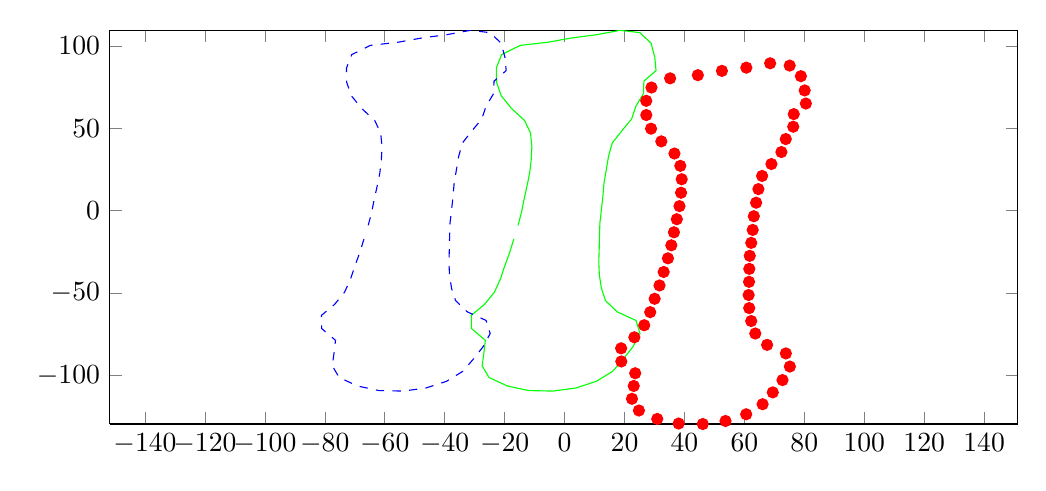
\begin{tikzpicture}

\begin{axis}[%
width=0.95092\figurewidth,
height=\figureheight,
at={(0\figurewidth,0\figureheight)},
scale only axis,
separate axis lines,
every outer x axis line/.append style={black},
every x tick label/.append style={font=\color{black}},
xmin=-151.778021214255,
xmax=151.161721492163,
every outer y axis line/.append style={black},
every y tick label/.append style={font=\color{black}},
ymin=-129.539052016635,
ymax=109.392454730847
]
\addplot [color=green,solid,forget plot]
  table[row sep=crcr]{%
-16.9383008024585	-17.2540700419669\\
-18.3191546519567	-25.4359033790996\\
-19.9491020291355	-33.5312106952851\\
-21.4291189738092	-41.6332714839577\\
-23.4325934348993	-49.5825754086476\\
-26.7176285471632	-56.8943991598107\\
-31.1267949632225	-63.5860197531732\\
-31.0704497227118	-71.5674748745803\\
-26.4379811698871	-78.7151426511731\\
-26.9284073326641	-86.4232733437989\\
-27.5110893006216	-94.2182867904342\\
-25.1979225333846	-101.328977289501\\
-19.0786164239692	-106.458107909618\\
-11.9329700175712	-109.235419234112\\
-3.87185321948764	-109.539052016635\\
3.69595476934701	-107.694550034826\\
10.6040509809237	-103.610505689942\\
16.0738264182722	-97.5033072431341\\
19.4667298360072	-90.3323944289307\\
22.7118143384688	-82.8716003330266\\
25.1758355250203	-74.6529650067753\\
23.8318526210809	-66.6897319700684\\
17.5728140268441	-61.4916681638731\\
13.6357941739749	-54.6124247953319\\
12.2743466048961	-47.0227345980446\\
11.6053154311707	-39.1855081988353\\
11.4141254579142	-31.2468930073932\\
11.5508054391741	-23.2526358624026\\
11.6382748738122	-15.3810106226617\\
11.7862124201461	-7.44925402870258\\
12.2836207078492	0.408014023438319\\
12.764595432433	8.27040489118245\\
13.1459674974322	16.5683453024354\\
13.914944379972	24.7830543694155\\
14.6768488234752	33.0339986121794\\
15.9132711362889	41.0247575333806\\
19.0171378907613	48.2554620111854\\
22.3522725115161	55.5234846116251\\
23.8081395520568	63.3970336029318\\
26.2875145747278	70.892388597312\\
26.4645056213721	78.5519041188589\\
30.5104952411306	84.9694154986342\\
30.1178420665977	92.9115504342284\\
28.8517396683747	101.570102952583\\
25.1130491911448	107.995981860857\\
18.5884874875498	109.392454730847\\
10.6498659785291	106.739128233057\\
2.50383074847667	104.799129433769\\
-5.53504215733932	102.184734870287\\
-14.7813514194023	100.254498070884\\
-21.0049392171998	94.6760255214926\\
-22.7604403189108	86.62589780194\\
-22.7256966435158	77.9871674146514\\
-21.1470194611919	69.7081370790496\\
-17.7203358905016	62.0065646594886\\
-13.3397436214445	54.6264358822352\\
-11.3752111213659	47.1455296342044\\
-10.9180819392748	39.0335197567964\\
-11.1341721230248	30.8260313769864\\
-11.6566897428528	22.7037005494587\\
-12.5495998431267	14.7548011008601\\
-13.51112615278	6.82423225112747\\
-14.3842506054937	-1.06404766792365\\
-15.5164439615494	-8.98008173430333\\
};
\addplot [color=red,only marks,mark=*,mark options={solid},forget plot]
  table[row sep=crcr]{%
33.0616991975415	-37.2540700419669\\
31.6808453480433	-45.4359033790996\\
30.0508979708645	-53.5312106952851\\
28.5708810261909	-61.6332714839577\\
26.5674065651007	-69.5825754086476\\
23.2823714528368	-76.8943991598107\\
18.8732050367775	-83.5860197531732\\
18.9295502772882	-91.5674748745803\\
23.5620188301129	-98.7151426511731\\
23.0715926673359	-106.423273343799\\
22.4889106993784	-114.218286790434\\
24.8020774666154	-121.328977289501\\
30.9213835760308	-126.458107909618\\
38.0670299824288	-129.235419234112\\
46.1281467805124	-129.539052016635\\
53.695954769347	-127.694550034826\\
60.6040509809237	-123.610505689942\\
66.0738264182722	-117.503307243134\\
69.4667298360072	-110.332394428931\\
72.7118143384688	-102.871600333027\\
75.1758355250203	-94.6529650067753\\
73.8318526210809	-86.6897319700684\\
67.5728140268441	-81.4916681638731\\
63.6357941739749	-74.6124247953319\\
62.2743466048961	-67.0227345980446\\
61.6053154311707	-59.1855081988353\\
61.4141254579142	-51.2468930073932\\
61.5508054391741	-43.2526358624026\\
61.6382748738122	-35.3810106226617\\
61.7862124201461	-27.4492540287026\\
62.2836207078492	-19.5919859765617\\
62.764595432433	-11.7295951088175\\
63.1459674974322	-3.43165469756458\\
63.914944379972	4.78305436941551\\
64.6768488234752	13.0339986121794\\
65.9132711362889	21.0247575333806\\
69.0171378907613	28.2554620111854\\
72.3522725115161	35.5234846116251\\
73.8081395520568	43.3970336029318\\
76.2875145747278	50.892388597312\\
76.4645056213721	58.5519041188589\\
80.5104952411306	64.9694154986342\\
80.1178420665977	72.9115504342284\\
78.8517396683747	81.5701029525829\\
75.1130491911449	87.9959818608571\\
68.5884874875498	89.3924547308472\\
60.6498659785291	86.7391282330572\\
52.5038307484767	84.7991294337689\\
44.4649578426607	82.1847348702868\\
35.2186485805977	80.2544980708841\\
28.9950607828002	74.6760255214926\\
27.2395596810892	66.62589780194\\
27.2743033564842	57.9871674146514\\
28.8529805388081	49.7081370790496\\
32.2796641094984	42.0065646594886\\
36.6602563785556	34.6264358822352\\
38.6247888786341	27.1455296342044\\
39.0819180607252	19.0335197567964\\
38.8658278769752	10.8260313769864\\
38.3433102571472	2.70370054945868\\
37.4504001568733	-5.2451988991399\\
36.48887384722	-13.1757677488725\\
35.6157493945063	-21.0640476679236\\
34.4835560384506	-28.9800817343033\\
};
\addplot [color=blue,dashed,forget plot]
  table[row sep=crcr]{%
-66.9383008024585	-17.2540700419669\\
-68.3191546519567	-25.4359033790996\\
-69.9491020291355	-33.5312106952851\\
-71.4291189738092	-41.6332714839577\\
-73.4325934348993	-49.5825754086476\\
-76.7176285471632	-56.8943991598107\\
-81.1267949632225	-63.5860197531732\\
-81.0704497227118	-71.5674748745803\\
-76.4379811698871	-78.7151426511731\\
-76.9284073326641	-86.4232733437989\\
-77.5110893006216	-94.2182867904342\\
-75.1979225333846	-101.328977289501\\
-69.0786164239692	-106.458107909618\\
-61.9329700175712	-109.235419234112\\
-53.8718532194876	-109.539052016635\\
-46.304045230653	-107.694550034826\\
-39.3959490190763	-103.610505689942\\
-33.9261735817278	-97.5033072431341\\
-30.5332701639928	-90.3323944289307\\
-27.2881856615312	-82.8716003330266\\
-24.8241644749797	-74.6529650067753\\
-26.1681473789191	-66.6897319700684\\
-32.4271859731559	-61.4916681638731\\
-36.3642058260251	-54.6124247953319\\
-37.7256533951039	-47.0227345980446\\
-38.3946845688293	-39.1855081988353\\
-38.5858745420858	-31.2468930073932\\
-38.4491945608259	-23.2526358624026\\
-38.3617251261878	-15.3810106226617\\
-38.2137875798539	-7.44925402870258\\
-37.7163792921508	0.408014023438319\\
-37.235404567567	8.27040489118245\\
-36.8540325025678	16.5683453024354\\
-36.085055620028	24.7830543694155\\
-35.3231511765248	33.0339986121794\\
-34.0867288637111	41.0247575333806\\
-30.9828621092387	48.2554620111854\\
-27.6477274884839	55.5234846116251\\
-26.1918604479432	63.3970336029318\\
-23.7124854252722	70.892388597312\\
-23.5354943786279	78.5519041188589\\
-19.4895047588694	84.9694154986342\\
-19.8821579334023	92.9115504342284\\
-21.1482603316253	101.570102952583\\
-24.8869508088552	107.995981860857\\
-31.4115125124502	109.392454730847\\
-39.3501340214709	106.739128233057\\
-47.4961692515233	104.799129433769\\
-55.5350421573393	102.184734870287\\
-64.7813514194023	100.254498070884\\
-71.0049392171998	94.6760255214926\\
-72.7604403189108	86.62589780194\\
-72.7256966435158	77.9871674146514\\
-71.1470194611919	69.7081370790496\\
-67.7203358905016	62.0065646594886\\
-63.3397436214444	54.6264358822352\\
-61.3752111213659	47.1455296342044\\
-60.9180819392748	39.0335197567964\\
-61.1341721230248	30.8260313769864\\
-61.6566897428528	22.7037005494587\\
-62.5495998431267	14.7548011008601\\
-63.51112615278	6.82423225112747\\
-64.3842506054937	-1.06404766792365\\
-65.5164439615494	-8.98008173430333\\
};
\end{axis}
\end{tikzpicture}%
					\caption{$t=(50,-20)$ (rot) und $t=(-50,0)$ (blau)}
					\label{fig:t}
				\end{subfigure}
				\qquad
				\begin{subfigure}{0.45\textwidth}
					\centering
					% This file was created by matlab2tikz.
% Minimal pgfplots version: 1.3
%
%The latest updates can be retrieved from
%  http://www.mathworks.com/matlabcentral/fileexchange/22022-matlab2tikz
%where you can also make suggestions and rate matlab2tikz.
%
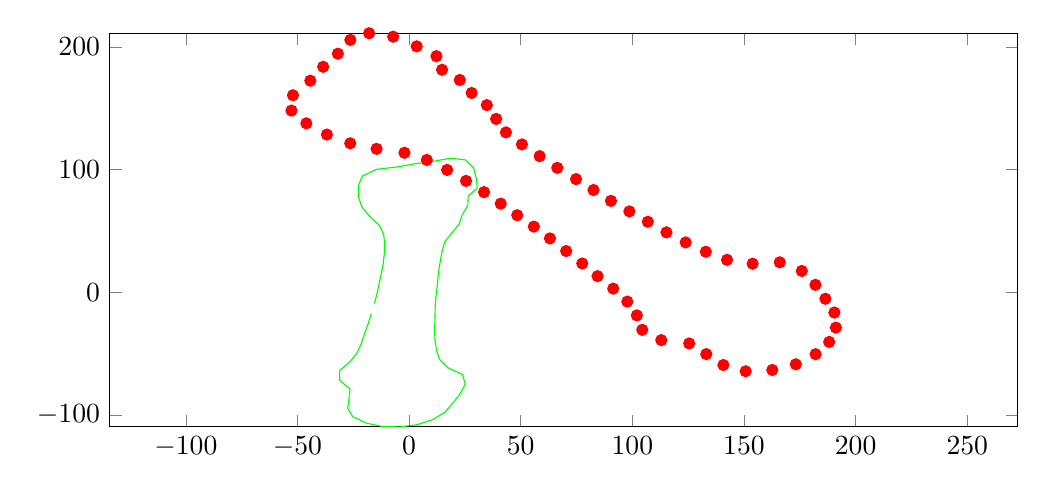
\begin{tikzpicture}

\begin{axis}[%
width=0.95092\figurewidth,
height=\figureheight,
at={(0\figurewidth,0\figureheight)},
scale only axis,
separate axis lines,
every outer x axis line/.append style={black},
every x tick label/.append style={font=\color{black}},
xmin=-134.098692432891,
xmax=272.543331799771,
every outer y axis line/.append style={black},
every y tick label/.append style={font=\color{black}},
ymin=-109.539052016634,
ymax=211.183447741062
]
\addplot [color=green,solid,forget plot]
  table[row sep=crcr]{%
-16.9383008024585	-17.2540700419669\\
-18.3191546519567	-25.4359033790996\\
-19.9491020291355	-33.5312106952851\\
-21.4291189738092	-41.6332714839577\\
-23.4325934348993	-49.5825754086476\\
-26.7176285471632	-56.8943991598107\\
-31.1267949632225	-63.5860197531732\\
-31.0704497227118	-71.5674748745803\\
-26.4379811698871	-78.7151426511731\\
-26.9284073326641	-86.4232733437989\\
-27.5110893006216	-94.2182867904342\\
-25.1979225333846	-101.328977289501\\
-19.0786164239692	-106.458107909618\\
-11.9329700175712	-109.235419234112\\
-3.87185321948764	-109.539052016635\\
3.69595476934701	-107.694550034826\\
10.6040509809237	-103.610505689942\\
16.0738264182722	-97.5033072431341\\
19.4667298360072	-90.3323944289307\\
22.7118143384688	-82.8716003330266\\
25.1758355250203	-74.6529650067753\\
23.8318526210809	-66.6897319700684\\
17.5728140268441	-61.4916681638731\\
13.6357941739749	-54.6124247953319\\
12.2743466048961	-47.0227345980446\\
11.6053154311707	-39.1855081988353\\
11.4141254579142	-31.2468930073932\\
11.5508054391741	-23.2526358624026\\
11.6382748738122	-15.3810106226617\\
11.7862124201461	-7.44925402870258\\
12.2836207078492	0.408014023438319\\
12.764595432433	8.27040489118245\\
13.1459674974322	16.5683453024354\\
13.914944379972	24.7830543694155\\
14.6768488234752	33.0339986121794\\
15.9132711362889	41.0247575333806\\
19.0171378907613	48.2554620111854\\
22.3522725115161	55.5234846116251\\
23.8081395520568	63.3970336029318\\
26.2875145747278	70.892388597312\\
26.4645056213721	78.5519041188589\\
30.5104952411306	84.9694154986342\\
30.1178420665977	92.9115504342284\\
28.8517396683747	101.570102952583\\
25.1130491911448	107.995981860857\\
18.5884874875498	109.392454730847\\
10.6498659785291	106.739128233057\\
2.50383074847667	104.799129433769\\
-5.53504215733932	102.184734870287\\
-14.7813514194023	100.254498070884\\
-21.0049392171998	94.6760255214926\\
-22.7604403189108	86.62589780194\\
-22.7256966435158	77.9871674146514\\
-21.1470194611919	69.7081370790496\\
-17.7203358905016	62.0065646594886\\
-13.3397436214445	54.6264358822352\\
-11.3752111213659	47.1455296342044\\
-10.9180819392748	39.0335197567964\\
-11.1341721230248	30.8260313769864\\
-11.6566897428528	22.7037005494587\\
-12.5495998431267	14.7548011008601\\
-13.51112615278	6.82423225112747\\
-14.3842506054937	-1.06404766792365\\
-15.5164439615494	-8.98008173430333\\
};
\addplot [color=red,only marks,mark=*,mark options={solid},forget plot]
  table[row sep=crcr]{%
70.3349238558198	33.7335140665925\\
77.5484519274452	23.5907526325438\\
84.4060017109704	13.2755623188774\\
91.4297398720799	3.11223410421886\\
97.7362443723151	-7.4442815281291\\
102.007298701771	-18.6839476705381\\
104.428206941549	-30.4581103268426\\
112.953581654153	-38.8639587344882\\
125.448303076902	-41.5317303752305\\
133.103834803388	-50.2276130978287\\
140.753667548495	-59.1135009553897\\
150.749177615401	-64.2020433009097\\
162.679946449202	-63.1518035963385\\
173.204832500613	-58.5184845579744\\
182.076989227674	-50.2904302294504\\
188.147471960235	-40.3071679191433\\
191.142831298277	-28.6482422282996\\
190.466742099567	-16.3690071196397\\
186.459558004123	-5.16438798042142\\
181.988122742568	6.19091105277499\\
175.884432720628	17.5215793447093\\
166.01263946223	24.542354327584\\
153.860547262089	23.4170206266458\\
142.388167655652	26.5377199261932\\
132.894052334753	33.1437688221152\\
123.871803716241	40.7467880013283\\
115.248843173715	48.9641733641003\\
106.914624029459	57.5883345331602\\
98.6582799960581	66.0302292576988\\
90.4022931479009	74.6000390324705\\
82.5959830258769	83.4615114742542\\
74.7668089114941	92.3109870566346\\
66.3700201694498	101.516788118627\\
58.4726285916749	111.045426001061\\
50.5293023517251	120.604995636862\\
43.3652465244142	130.391899269576\\
38.988074115877	141.353367368074\\
34.8166164757535	152.599713927715\\
28.0096368354258	162.495053938659\\
22.6893866569886	173.074852792002\\
14.7529709620917	181.386723194773\\
12.2375922847326	192.484941962357\\
3.39721449609688	200.492376583893\\
-7.12947169257571	208.333253998186\\
-17.9106256030724	211.183447741062\\
-26.3121514945651	205.744288157908\\
-31.918053409084	194.509830765522\\
-38.5005490758102	183.811976179384\\
-44.2540772062059	172.512479675382\\
-52.0139438812048	160.657962409923\\
-52.6981919313969	148.139987054717\\
-46.0217321816272	137.739547104747\\
-36.8221236923734	128.613641080918\\
-26.3664459430552	121.506843354377\\
-14.5631480328253	116.972639013594\\
-2.08901962759099	113.791150105551\\
7.92938105751433	107.940152178446\\
17.0183255643679	99.8209251051973\\
25.4944833477618	90.886370818971\\
33.5553025301352	81.7171243797881\\
41.0393094044059	72.3389691448366\\
48.4310952621072	62.9074779655997\\
55.8717912640948	53.6146052996112\\
63.067140917234	44.017510847428\\
};
\end{axis}
\end{tikzpicture}%
					\caption{$s=1.5$, $r=45^\circ$ und $t=(70,70)$ (rot)}
					\label{fig:mix}
				\end{subfigure}	
				\caption{Vergleich zwischen transformierten Shapes mit Vergrößerungsfaktor $s$, Drehwinkel $r$ und Translationsvektor $t=(t_x,t_y)$ und Original-Shape (grün, $s=1$, $r=0$, $t=(0,0)$) : Skalierung~(\ref{fig:s}), Rotation~(\ref{fig:r}), Translation~(\ref{fig:t}) und beliebige Transformation~(\ref{fig:mix}).}
				\label{fig:trafo}
			\end{figure}
			

		\item Featureberechnung
			
		\item Klassifikation und Feature-Selection
			\begin{enumerate}
				\setcounter{enumii}{1}
				\item TODO: oobError
				\item TODO: oobVar
			\setlength\figureheight{3.5cm}
			\setlength\figurewidth{\textwidth}
				\begin{figure}
					%\begin{subfigure}{0.7\textwidth}
					\centering
					\includegraphics[height=3.5cm]{figures/OOBErr.png}
					%% This file was created by matlab2tikz.
% Minimal pgfplots version: 1.3
%
%The latest updates can be retrieved from
%  http://www.mathworks.com/matlabcentral/fileexchange/22022-matlab2tikz
%where you can also make suggestions and rate matlab2tikz.
%
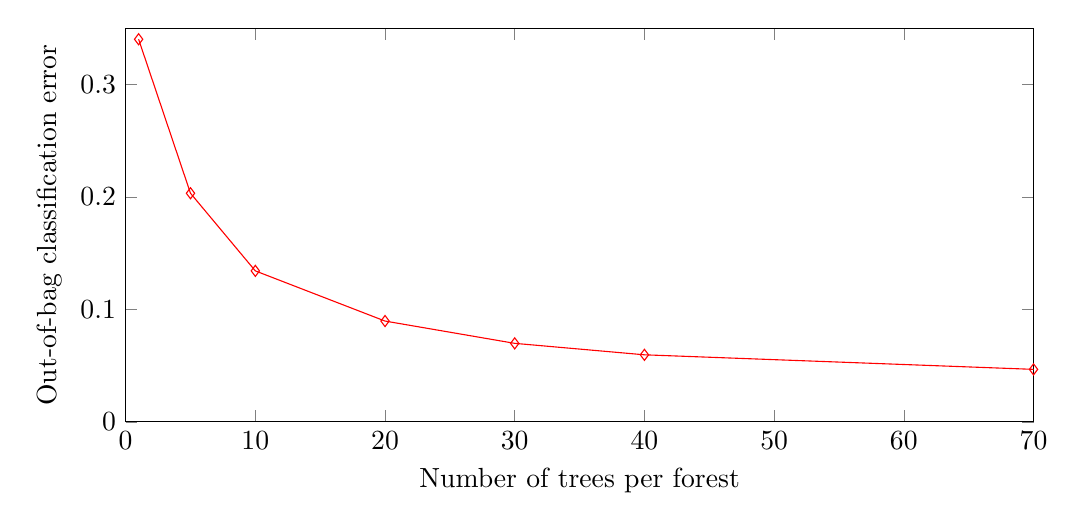
\begin{tikzpicture}

\begin{axis}[%
width=0.95092\figurewidth,
height=\figureheight,
at={(0\figurewidth,0\figureheight)},
scale only axis,
separate axis lines,
every outer x axis line/.append style={black},
every x tick label/.append style={font=\color{black}},
xmin=0,
xmax=70,
xlabel={Number of trees per forest},
every outer y axis line/.append style={black},
every y tick label/.append style={font=\color{black}},
ymin=0,
ymax=0.35,
ylabel={Out-of-bag classification error}
]
\addplot [color=red,solid,mark=diamond,mark options={solid},forget plot]
  table[row sep=crcr]{%
1	0.340200089496886\\
5	0.203289011059243\\
10	0.134262929105653\\
20	0.0896710988940598\\
30	0.0698512646764143\\
40	0.0596664642331929\\
70	0.0467338197824591\\
};
\end{axis}
\end{tikzpicture}%
					\caption{Classification error for different numbers of trees per forest}
					\label{fig:oobErr}
					%\end{subfigure}
					\qquad
					%\begin{subfigure}{0.7\textwidth}
					\centering
					\includegraphics[width=\textwidth,height=4cm]{figures/OOBVarStacked.png}
					\caption{Feature importance for different number of trees per forest}
					\label{fig:oobVar}
					%\end{subfigure}
				\end{figure}
			\end{enumerate}
		
		\item Shape Particle Filter
			\begin{enumerate}
				\setcounter{enumii}{3}
				\item
				
				\setlength\figureheight{3.5cm}
				\setlength\figurewidth{.4\textwidth}
				\begin{figure}
%					\begin{subfigure}{0.45\textwidth}
%						\centering
%%						\input{}
%						\caption{}
%						\label{fig:box_9EV_dist_gross}
%					\end{subfigure}
%					\qquad
%					\begin{subfigure}{0.45\textwidth}
%						\centering
%						% This file was created by matlab2tikz.
% Minimal pgfplots version: 1.3
%
%The latest updates can be retrieved from
%  http://www.mathworks.com/matlabcentral/fileexchange/22022-matlab2tikz
%where you can also make suggestions and rate matlab2tikz.
%
\begin{tikzpicture}

\begin{axis}[%
width=0.95092\figurewidth,
height=\figureheight,
at={(0\figurewidth,0\figureheight)},
scale only axis,
xmin=0.5,
xmax=1.5,
xtick={1},
xticklabels={{95% variance within model}},
ymin=-0.728566884339413,
ymax=15.9466402995033,
ylabel={distance from landmark to nearest mask point [pixel]},
title style={font=\bfseries},
title={segmentation performance of the model}
]
\addplot [color=black,dashed,forget plot]
  table[row sep=crcr]{%
1	2.04667757757944\\
1	4.34318954716592\\
};
\addplot [color=black,dashed,forget plot]
  table[row sep=crcr]{%
1	0.0293970785625268\\
1	0.50798954945933\\
};
\addplot [color=black,solid,forget plot]
  table[row sep=crcr]{%
0.9625	4.34318954716592\\
1.0375	4.34318954716592\\
};
\addplot [color=black,solid,forget plot]
  table[row sep=crcr]{%
0.9625	0.0293970785625268\\
1.0375	0.0293970785625268\\
};
\addplot [color=blue,solid,forget plot]
  table[row sep=crcr]{%
0.925	0.50798954945933\\
0.925	2.04667757757944\\
1.075	2.04667757757944\\
1.075	0.50798954945933\\
0.925	0.50798954945933\\
};
\addplot [color=red,solid,forget plot]
  table[row sep=crcr]{%
0.925	1.02359763520799\\
1.075	1.02359763520799\\
};
\addplot [color=black,only marks,mark=+,mark options={solid,draw=red},forget plot]
  table[row sep=crcr]{%
1	4.39245868034132\\
1	4.39853519130335\\
1	4.41542718339205\\
1	4.44278253858104\\
1	4.44511415894837\\
1	4.45409429769892\\
1	4.45412636851505\\
1	4.45935823946378\\
1	4.46178886372344\\
1	4.51311199809143\\
1	4.51698147233412\\
1	4.52394877390238\\
1	4.52790778621183\\
1	4.5310388105982\\
1	4.5512484583238\\
1	4.66676907106546\\
1	4.67820118698629\\
1	4.73673492306747\\
1	4.78656992091044\\
1	4.78714397170129\\
1	4.87599920670225\\
1	4.92916198741749\\
1	4.94557014740897\\
1	4.96144267769778\\
1	5.06274343568621\\
1	5.08137614160822\\
1	5.08723508899509\\
1	5.09635949830619\\
1	5.22557417316904\\
1	5.22969988117126\\
1	5.257527019242\\
1	5.31161414774427\\
1	5.46957724954451\\
1	5.60938566483263\\
1	5.65724571356633\\
1	5.74392034093735\\
1	5.74982764060428\\
1	5.75455861309482\\
1	5.76865363498537\\
1	5.77683997873468\\
1	5.78425261689584\\
1	5.79244315358018\\
1	5.83700048068328\\
1	5.8438746826321\\
1	5.89437512075632\\
1	5.9136621504401\\
1	6.00565833075111\\
1	6.06947776944622\\
1	6.07148095587123\\
1	6.08845718886048\\
1	6.16702669255058\\
1	6.25652506575766\\
1	6.28653785176343\\
1	6.28861898070952\\
1	6.30594434816903\\
1	6.32795777869356\\
1	6.5162744001749\\
1	6.52150204588923\\
1	6.54416371642653\\
1	6.59231036703585\\
1	6.64129126490008\\
1	6.67268820916965\\
1	6.71573332719001\\
1	6.93952764910191\\
1	6.98935728589379\\
1	7.14557152785841\\
1	7.17397761100275\\
1	7.19335282383802\\
1	7.21417792128503\\
1	7.38458607600278\\
1	7.49882669488107\\
1	7.51349740666094\\
1	7.52702622542253\\
1	7.62247858612681\\
1	7.72002080691356\\
1	7.80057877544884\\
1	7.91327137040607\\
1	7.98158353147495\\
1	8.00311250250357\\
1	8.02760153472465\\
1	8.02961434018828\\
1	8.06749291163842\\
1	8.51415121202003\\
1	9.02756583725783\\
1	9.36133601130487\\
1	9.67151683319852\\
1	10.0519537515251\\
1	10.101959830275\\
1	10.1651764613481\\
1	10.3714607733995\\
1	10.5838860692452\\
1	10.7708142067919\\
1	11.1047122754382\\
1	11.4988306962536\\
1	11.8235757442374\\
1	11.8385705395526\\
1	15.0326165295625\\
1	15.1886763366013\\
};
\end{axis}
\end{tikzpicture}%
%						\caption{test}
%						\label{fig:box_4EV_dist_gross}
%					\end{subfigure}	
%					\\
%					\begin{subfigure}{0.45\textwidth}
%						\centering
%%						\input{}
%						\caption{}
%						\label{fig:box_9EV_bool_gross}
%					\end{subfigure}
%					\qquad
%					\begin{subfigure}{0.45\textwidth}
%						\centering
%%						\input{}
%						\caption{}
%						\label{fig:box_9EV_dist_klein}
%					\end{subfigure}	
					\caption{}
					\label{fig:box}
				\end{figure}
			\end{enumerate}
			
	\end{enumerate}
	
\end{document}          
